\begin{figure}[ht]
    \centering
    \begin{subfigure}{0.24\textwidth}
        \centering
        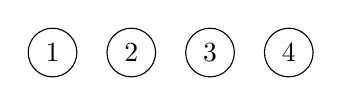
\begin{tikzpicture}[scale=1, every node/.style={circle,draw,minimum size=5mm}]
            \node (n0) at (0,0) {1};
            \node (n1) at (1,0) {2};
            \node (n3) at (2,0) {3};
            \node (n4) at (3,0) {4};
        \end{tikzpicture}
        \caption{Krok 1}
        \label{fig:disjoint_set_a}
    \end{subfigure}
    \begin{subfigure}{0.24\textwidth}
        \centering
        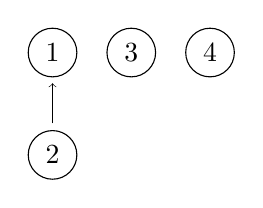
\begin{tikzpicture}[scale=1, every node/.style={circle,draw,minimum size=5mm}]
            \node (n0) at (0,1.3) {1};
            \node (n1) at (0,0) {2};
            \node (n2) at (1,1.3) {3};
            \node (n3) at (2,1.3) {4};
            \draw[->, very thin, black] (0,0.4) -- (0,0.91);
        \end{tikzpicture}
        \caption{Krok 2}
        \label{fig:disjoint_set_b}
    \end{subfigure}
    \begin{subfigure}{0.24\textwidth}
        \centering
        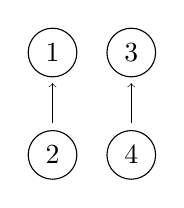
\begin{tikzpicture}[scale=1, every node/.style={circle,draw,minimum size=5mm}]
            \node (n0) at (0,1.3) {1};
            \node (n1) at (0,0) {2};
            \node (n2) at (1,1.3) {3};
            \node (n3) at (1,0) {4};
            \draw[->, very thin, black] (0,0.4) -- (0,0.91);
            \draw[->, very thin, black] (1,0.4) -- (1,0.91);
        \end{tikzpicture}
        \caption{Krok 3}
        \label{fig:disjoint_set_c}
    \end{subfigure}
    \hfill
    \begin{subfigure}{0.24\textwidth}
        \centering
        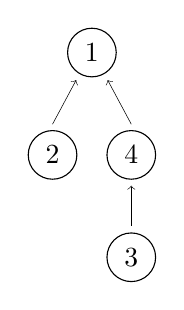
\begin{tikzpicture}[scale=1, every node/.style={circle,draw,minimum size=5mm}]
            \node (n0) at (0.5,2.6) {1};
            \node (n1) at (0,1.3) {2};
            \node (n2) at (1,0) {3};
            \node (n3) at (1,1.3) {4};
            \draw[->, very thin, black] (0,1.69) -- (0.3,2.25);
            \draw[->, very thin, black] (1,1.69) -- (0.7,2.25);
            \draw[->, very thin, black] (1,0.4) -- (1,0.91);
        \end{tikzpicture}
        \caption{Krok 4}
        \label{fig:disjoint_set_d}
    \end{subfigure}
    \caption{Kolejne kroki scalania zbioru}
    \label{fig:disjoint_set}
\end{figure}
%https://cp-algorithms.com/data_structures/disjoint_set_union.html